\section{Launch The Simulation}

\begin{frame}[fragile]
	\frametitle{Launch Simulation Environment}
	In order to launch the simulation environment a ROS launch file is provided. Do the following command:
\begin{lstlisting}[language=bash]
$ roslaunch turtlebot3_autorace_simulation gazebo.launch
\end{lstlisting}

This launch file could take four input arguments:
\begin{itemize}
	\item \texttt{x\_pos}: set the x start coordinate of the robot
	\item \texttt{y\_pos}: set the y start coordinate of the robot
	\item \texttt{z\_pos}: set the z start coordinate of the robot
	\item \texttt{track}: set the track to import in the environment
\end{itemize}
By default it set $x = 0, y = 0, z = 0$ and set the track as \texttt{track1}
\end{frame}

\begin{frame}[fragile]
\frametitle{Launch Simulation Environment II}
Here is an example on how to launch the simulation with a different track:
\begin{lstlisting}[language=bash]
$ roslaunch turtlebot3_autorace_simulation gazebo.launch track:=track2
\end{lstlisting}
\begin{figure}
	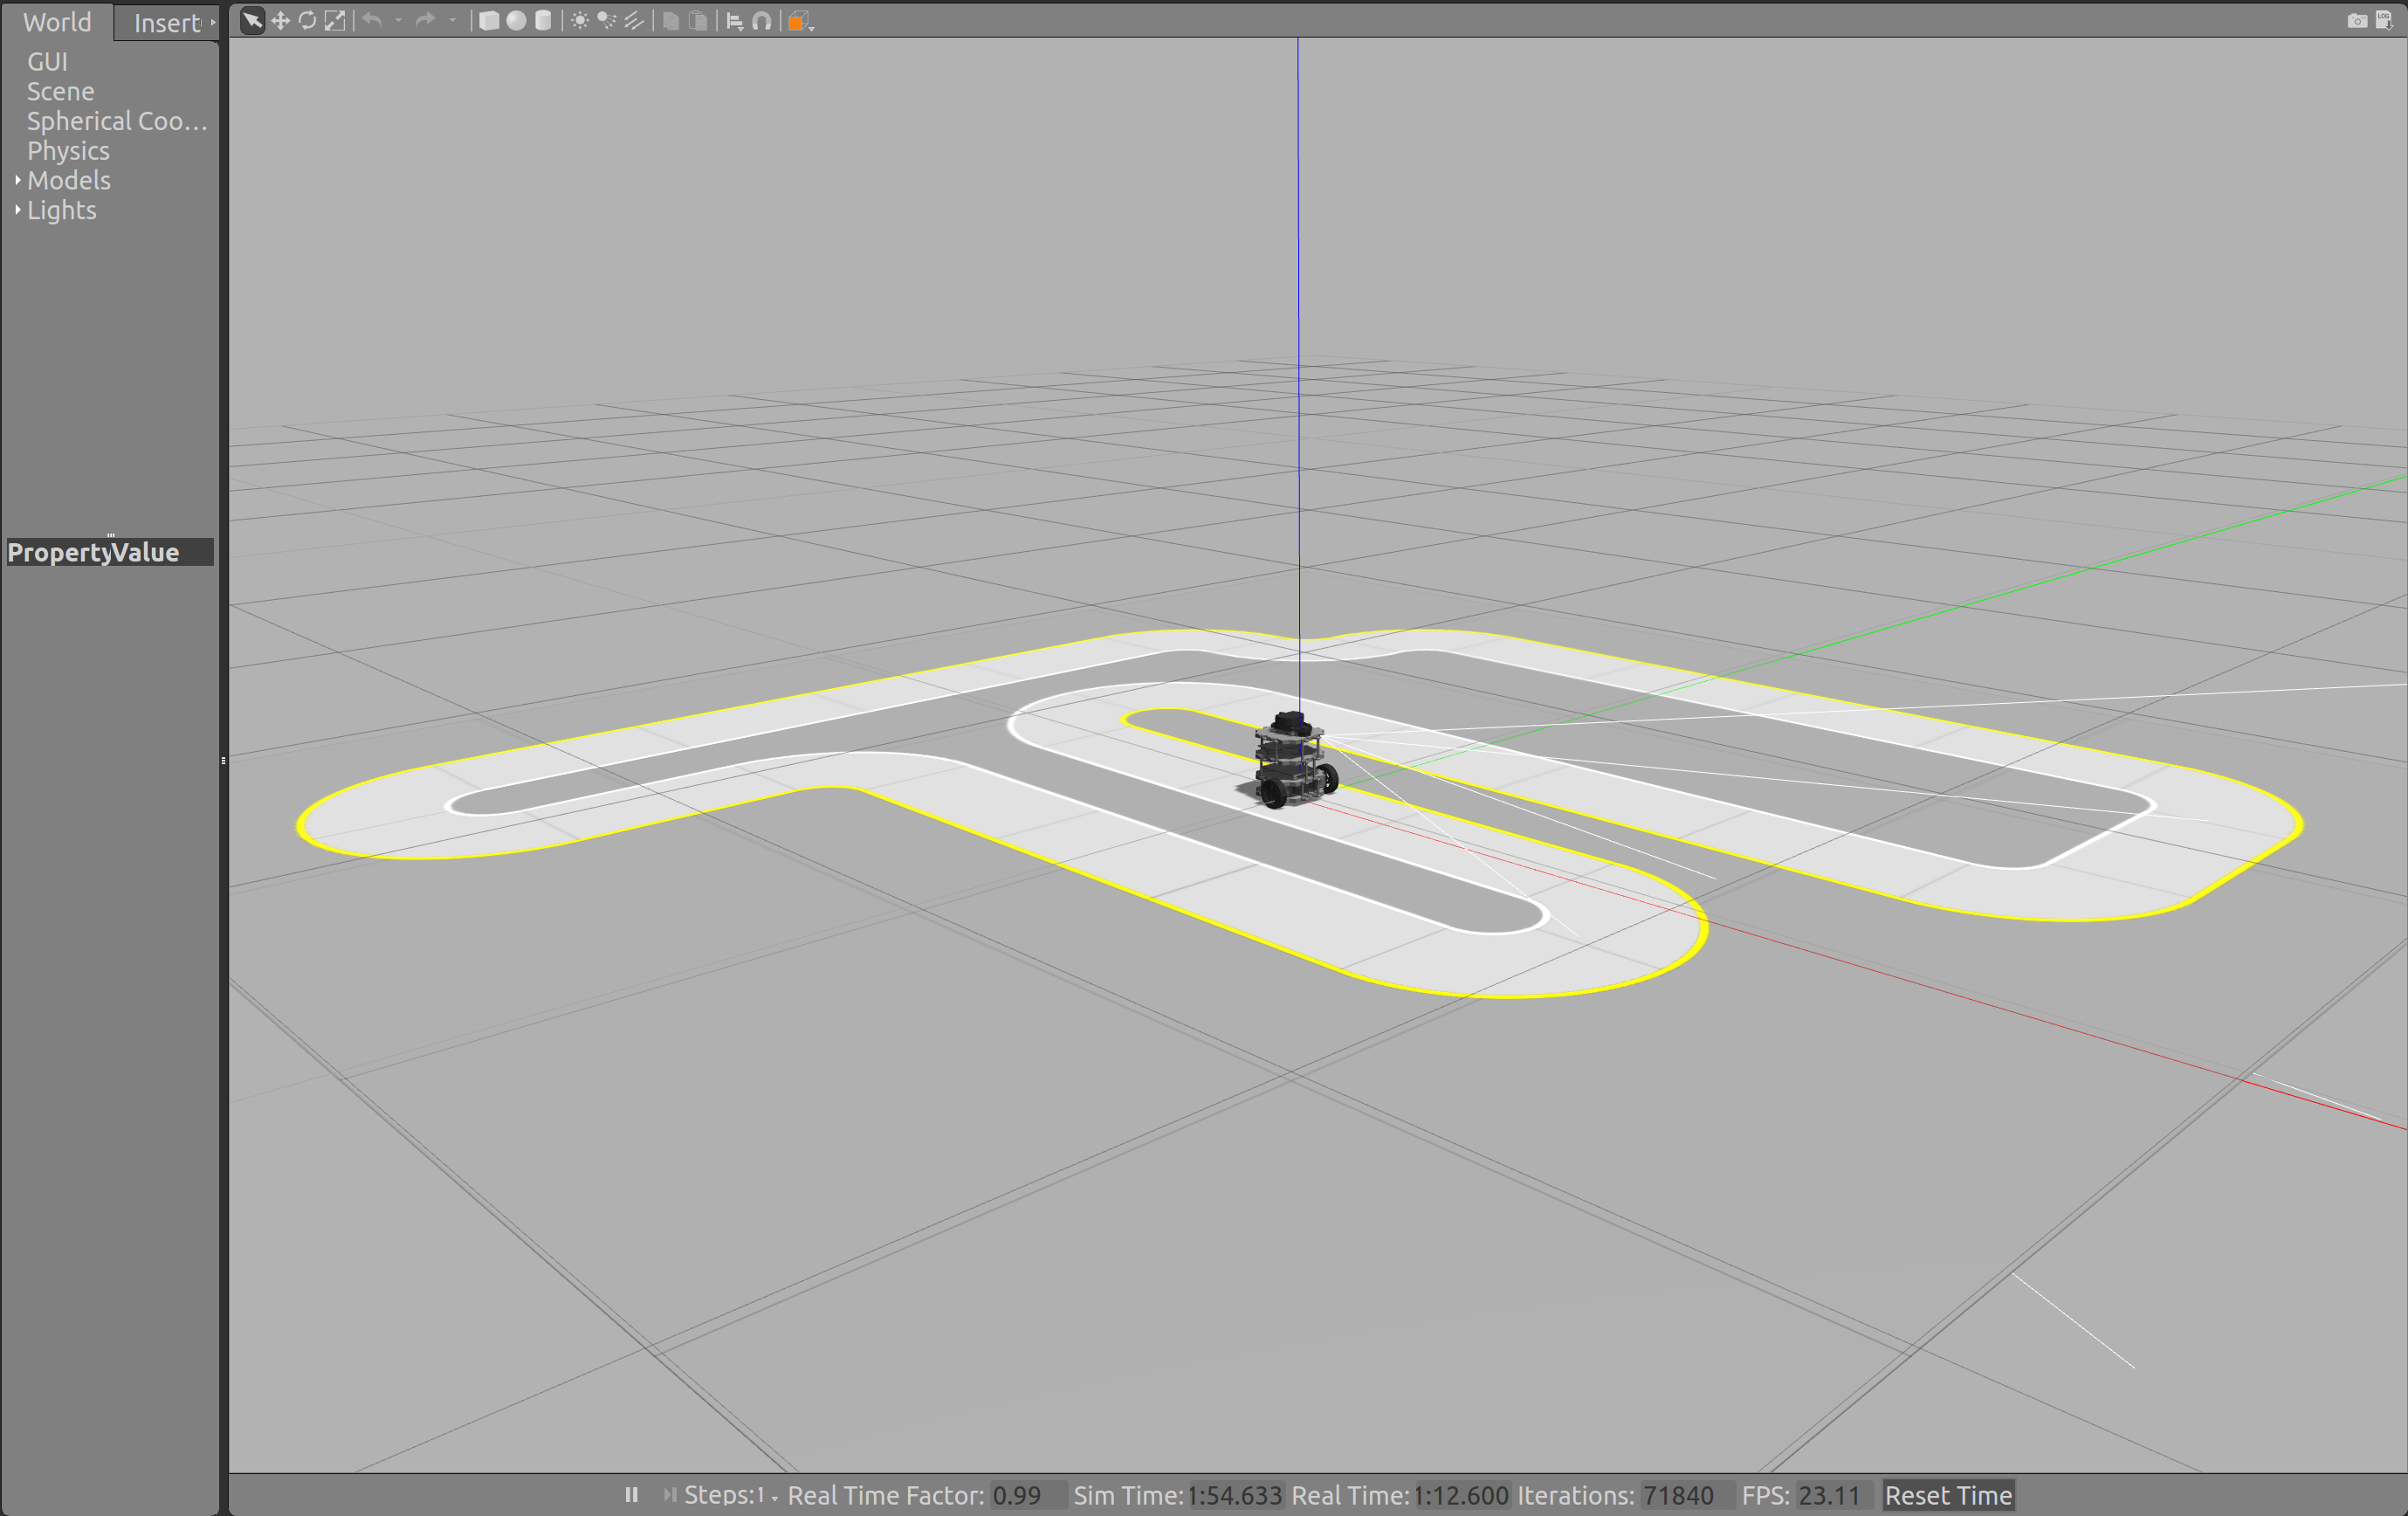
\includegraphics[width=0.7\textwidth]{figures/png/gazebo}
\end{figure}
\end{frame}

\begin{frame}[fragile]
	\frametitle{Launch Autodrive Nodes}
	In order to launch the Autodrive nodes a ROS launch file is provided. Do the following command:
\begin{lstlisting}[language=bash]
$ roslaunch turtlebot3_autorace_simulation autorace.launch
\end{lstlisting}

The calibration mode could be enabled by running the following command:
\begin{lstlisting}[language=bash]
$ roslaunch turtlebot3_autorace_simulation autorace.launch calibration_mode:=calibration
\end{lstlisting}
\end{frame}
